\documentclass{report}
\usepackage[utf8]{inputenc}
\usepackage{fixlatvian}
\usepackage{tabularx}
\usepackage{graphicx}
\usepackage{verbatim}
\usepackage[siunitx, europeanresistors, americaninductors, oldvoltagedirection]{circuitikz}
\usepackage{pgfplots}
\usepackage[document]{ragged2e}

\title{Vienkāršu elektrisku shēmu modelēšana}
\author{Inguss Pumpurs REBM02 }
\date{9.03.2018. - 23.03.2018.}

\begin{document}
\maketitle
%=====================

\chapter{Teorētiskā daļa}
\section{Ķēdes aprēķins}
\label{theory:circuit}

\justify
Tiek dota shēma, kurā ir jāaprēķina spriegumi uz rezistoriem. Par sprieguma avota V1 sprieguma vērtību U izmanto studenta apliecības pēdējos 3 ciparus, kas izdalīti ar 10, piemēram, 158, tādējādi V1 = 15.8. Rezistoru vērtības izvēlās šādi: R1 = studentu apliecības pirmspēdējais cipars + 1 (5+1=6, R1 = 6$\Omega$), R2 = studentu apliecības pēdējais cipars + 1 (8+1=9, R2 = 9$\Omega$). Aprēķina gaitu piefiksē un tālāk izmanto šajā darbā priekš aprēķiniem, kuru rezultāti ir redzami \ref{tab:1} tabulā.

\begin{equation}
    I=\frac{U}{R1+R2}
    \label{oms}
\end{equation}

\begin{equation}
    I=\frac{15.8}{6+9}=1.053 A
\end{equation}

\begin{table}[b!]
    \centering
    \begin{tabular}{|c|r|}
        \hline
        R1 & 6$\Omega$ \\
        \hline
        R2 & 9$\Omega$ \\
        \hline
        V1 & 15.8 V \\
        \hline
        $U_{R1}$ & 6.32 V \\
        \hline
        $U_{R2}$ & 9.48 V \\
        \hline
    \end{tabular}
    \captionof{table}{Aprēķinu rezultātu tabula}\label{tab:1}
\end{table}


\begin{figure}
    \centering
        \begin{circuitikz}[scale=1, every node/.style={transform shape}]
        \draw
        (0,2) to[R=$R1$, -] (4,2)
        (4,2) to[R=$R2$, -] (4,0)
        (0,0) to[short, -] (4,0)
        (0,0) to[american voltage source, v<=$V1$, -] (0,2);
    \end{circuitikz}
\caption{Dotās shēmas attēlojums ar "circuitikz" pakas palīdzību.}\label{sch:1}
\end{figure}

\begin{figure}
    \centering
        \begin{tikzpicture}
            \begin{axis}[
                xlabel=$R2$,
                ylabel=$U_{R2}$
                ]
            \addplot[color=red,mark=o] coordinates {
            		(0,0)
            		(1,2.26)
            		(2,3.95)
            		(3,5.27)
            		(4,6.32)
            		(5,7.18)
            		(6,7.9)
            		(7,8.51)
            		(8,9.03)
            		(9,9.48)
            	};
            \end{axis}
        \end{tikzpicture}
    \caption{$U_{R2}$=\textit{f}(\textit{R2}) grafiks pēc Sweep simulācijas datiem.}\label{plot:1}
\end{figure}

%=====================

\chapter{Praktiskā daļa}
\section{Darbs ar GEDA programmām}

\subsection{Darbs ar gschem}
Gschem darba rezultāts jeb shēma ir redzama \ref{att:gschem} attēlā.
\begin{figure}[b!]
    \centering
    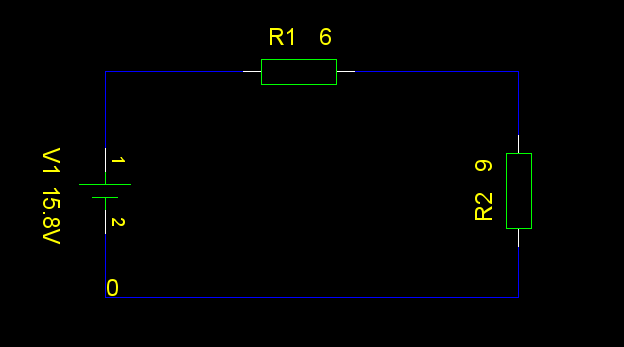
\includegraphics[width=10cm]{01.png}
    \captionof{figure}{Lietotnē gschem veidotā shēma}\label{att:gschem}
\end{figure}

\newpage
\subsection{Darbs ar gnetlist}
\begin{verbatim}
    * P01 Inguss Pumpurs
    V1 2 0 15.8V
    R2 0 1 9
    R1 2 1 6
    .END
\end{verbatim}


\subsection{Darbs ar ngspice}
\begin{figure}[b!]
    \centering
        \begin{minipage}{.5\textwidth}
        \centering
        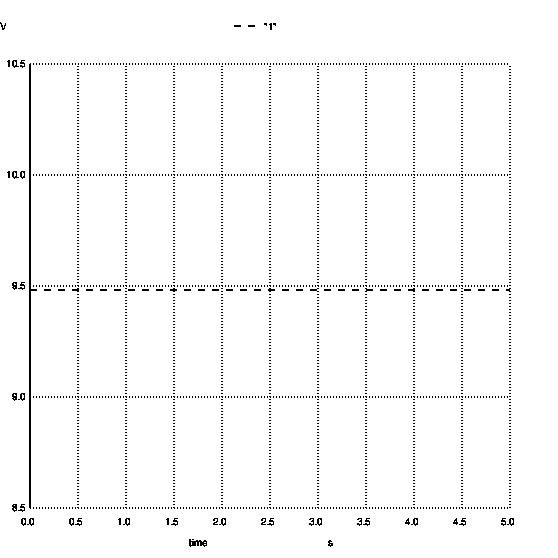
\includegraphics[width=6cm]{011.png}
        \captionof{figure}{Spriegums uz "1." vada pret "zemi"}
        \label{att:ngspice1}
        \end{minipage}%
        
        \begin{minipage}{.5\textwidth}
        \centering
        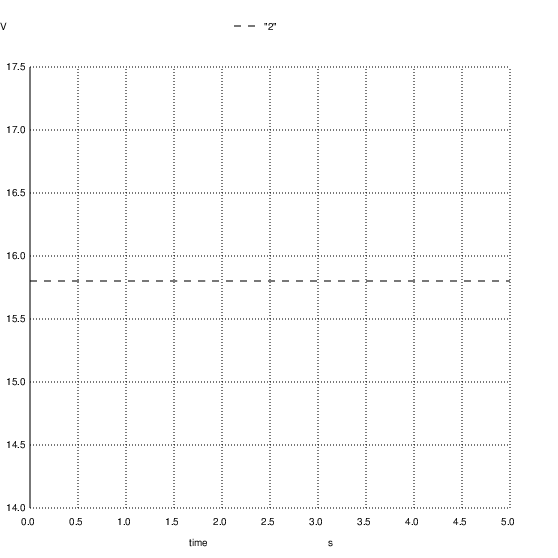
\includegraphics[width=6cm]{012.png}
        \captionof{figure}{Spriegums uz "2." vada pret "zemi"}
        \label{att:ngspice2}
        \end{minipage}
\end{figure}

\newpage

\section{Darbs ar QUCS programmām}
    \subsection{Principiālā shēma}
        \begin{figure}[b!]
            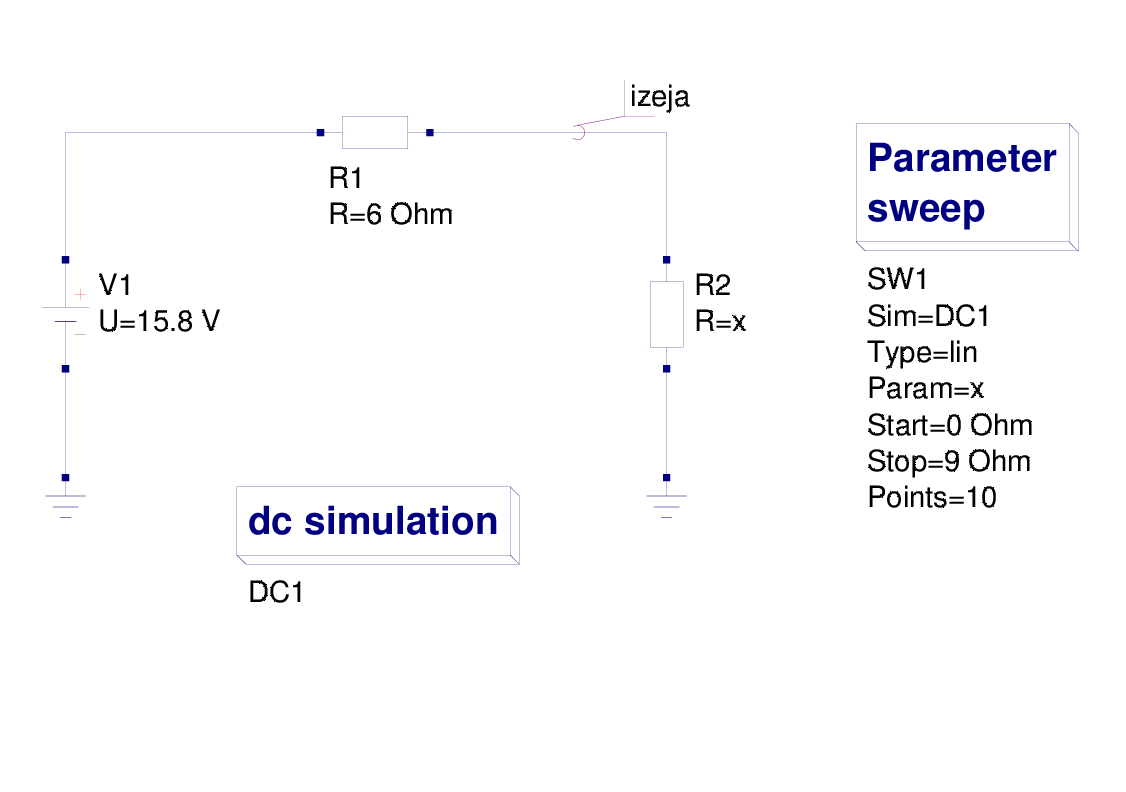
\includegraphics[scale=0.35]{02.png}
            \caption{Principiālā shēma}
            \label{att:qucs1}
        \end{figure}
       
        \justify
       \ref{att:qucs1} attēlā redzama tā pati shēma, kas bija redzama iepriekš sadaļā "Darbs ar gschem", tikai šoreiz QUCS izpildījumā. Kā redzams, R2 vērtībā ir ievietots mainīgais x, kurš tiek mainīts intervālā [0:9], ar kā palīdzību simulācijā būs iespējams iegūt līdzstrāvas un sweep simulāciju grafikus un sweep simulācijas tabulu. Sprieguma avots (V1) paliek nemainīgs, t.i., 15.8 V un R1 = 6 $\Omega$.
     
    
\newpage
   
   \subsection{DC un Sweep simulāciju rezultāti} 
    \begin{figure}[b!]
      \begin{center}
        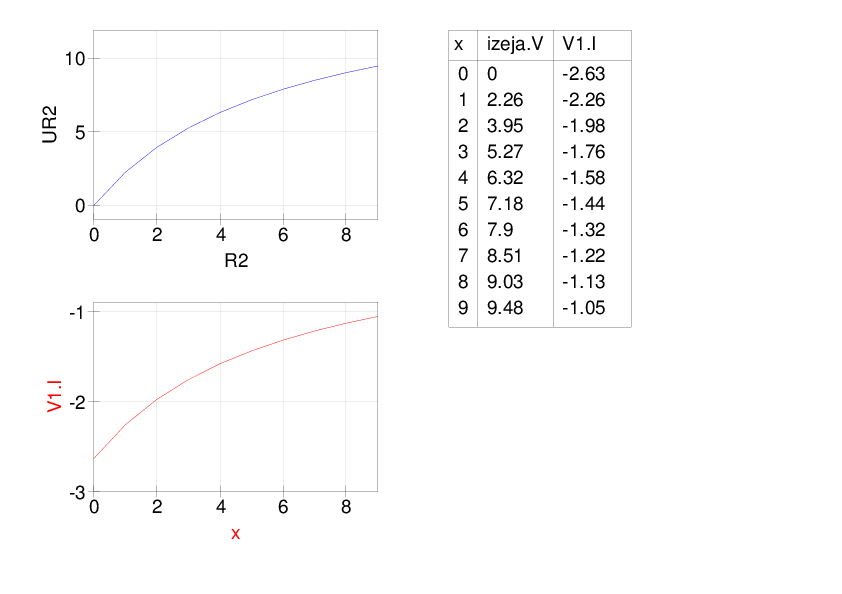
\includegraphics[scale=0.45]{022.png}
      \end{center}
      \caption{DC un Sweep simulāciju grafiki un tabula}
      \label{att:qucs2}
    \end{figure}
    
\justify
  \ref{att:qucs2} attēla pirmajā grafikā ir redzama $U_{R2}$ izmaiņa atkarībā no R2.
  
  \smallskip

\justify
  \ref{att:qucs2} attēla pirmajā grafikā ir redzams Sweep simulācijas grafiks. Pēc Sweep simulācijas(\ref{att:qucs2} attēlā redzamajā tabulā) rezultātiem var redzēt, ka, R2 vērtībai mainoties no 0 $\Omega$ līdz 9 $\Omega$ (saistībā ar \pageref{theory:circuit} teorētiskajā daļā minētajā ķēdes aprēķinā) spriegums izejas punktā palielinās atkarībā no R2 vērtības. Jo lielāka ir R2 vērtība, jo lielāks izejas spriegums. 
    
\chapter{Secinājumi}
\begin{itemize}
    \item Darbos līdz šim apguvu darbu ar Github, ķēžu modelēšanas programmām gschem\cite{geda} un QUCS, kā arī simulācijas programmu ngspice.
    \item Šajā darbā padziļinātāk apguvu \LaTeX dokumentēšanas valodu un tajā iekļauto bibliotēku iespējas, piemēram, ķēžu modelēšanu ar Circuitikz palīdzību.
    \item Apguvu online \LaTeX valodas redaktoru "ShareLatex".
    \item Veicu pirmā laboratorijas darba atskaiti.
\end{itemize}
    
\begin{thebibliography}{1}
\bibitem{Oms}
"Resistance to Ohm's Law", Morton L. Schagrin, American Journal of Physics (July 1963)
\bibitem{geda}
"Creating Open Source Electronic Hardware with Open Source Software", Tom Anderson (2008)
\end{thebibliography}

\end{document}
